%% content.tex
%%

%% ==============
\chapter{Content Chapters}
\label{ch:Content1}
%% ==============

% The content chapters of your thesis should of course be renamed. How many chapters you need to write depends on your thesis and cannot be said in general.

%  Always reference figures, tables etc. To give a few simple examples, this section contains Algorithm \ref{theorem:doof}, Table \ref{tbl:randomnumbers}, Figure \ref{fig:somegraph}, and Theorem \ref{theorem:doof}. To give an example citation we recommend the book of Garey and Johnson \cite{gj-ci-79}.

% \begin{algorithm}[bt]
% \caption{\textsc{Dijkstra}}\label{alg:dijkstra}

% % Some settings
% \DontPrintSemicolon %dontprintsemicolon
% \SetFuncSty{textsc}
% \SetKwFor{ForAll}{forall}{do}

% % Declaration of data containers and functions
% \SetKwData{Q}{Q}
% \SetKwData{dist}{d}
% \SetKwData{pred}{pred}
% \SetKwFunction{queueDeleteMin}{deleteMin}
% \SetKwFunction{queueInsert}{insert}
% \SetKwFunction{queueDecreaseKey}{decreaseKey}
% \SetKwFunction{queueContains}{contains}

% % Algorithm interface
% \KwIn{Graph $G = (V,E,\omega)$, source node $s$}
% \KwData{Priority queue \Q}
% \KwOut{Distances \dist{$v$} for all $v \in V$, shortest-path tree of $s$ given by \pred{$\cdot$}}

% % The algorithm
% \BlankLine
% \tcp{Initialization}
% \ForAll{$v \in V$}{$\dist{v} \leftarrow \infty$ \; $\pred{v} \leftarrow \texttt{null}$}
% \Q.\queueInsert{$s,0$}\; $\dist{s} \leftarrow 0$ \;
% \BlankLine
% \tcp{Main loop}
% \While{\Q is not empty}
% {
%   $u \leftarrow$ \Q.\queueDeleteMin{} \;
%   \ForAll{ $(u,v) \in E$ }
%   {
%     \If{$\dist{u} + \omega(u,v) < \dist{v}$}
%     {
%       $\dist{v} \leftarrow \dist{u} + \omega(u,v)$ \;
%       $\pred{v} \leftarrow u$ \;
%       \uIf{\Q.\queueContains{v}}
%       {
%         \Q.\queueDecreaseKey{$v, \dist{v}$}
%       }
%       \Else
%       {
%         \Q.\queueInsert{$v, \dist{v}$}
%       }
%     }
%   }
% }
% \end{algorithm}

% \begin{table} [bt]
% \centering
% \caption{Some strange numbers.}
% \begin{tabular}{rr}
% \toprule
% First column & Second column \\
% \midrule
% 3\,109\,218\,136 & 3\,208\,415\,108 \\
% 2\,231\,385\,058 & 1\,959\,477\,358 \\
% 1\,287\,719\,872 & 1\,317\,165\,206 \\
% 2\,516\,844\,936 & 2\,630\,583\,944 \\
% 1\,569\,466\,774 & 1\,636\,507\,220 \\
% 1\,032\,627\,816 &    991\,322\,491 \\
% \bottomrule
% \end{tabular}
% \label{tbl:randomnumbers}
% \end{table}

% \begin{figure} [bt]
%   \centering
%   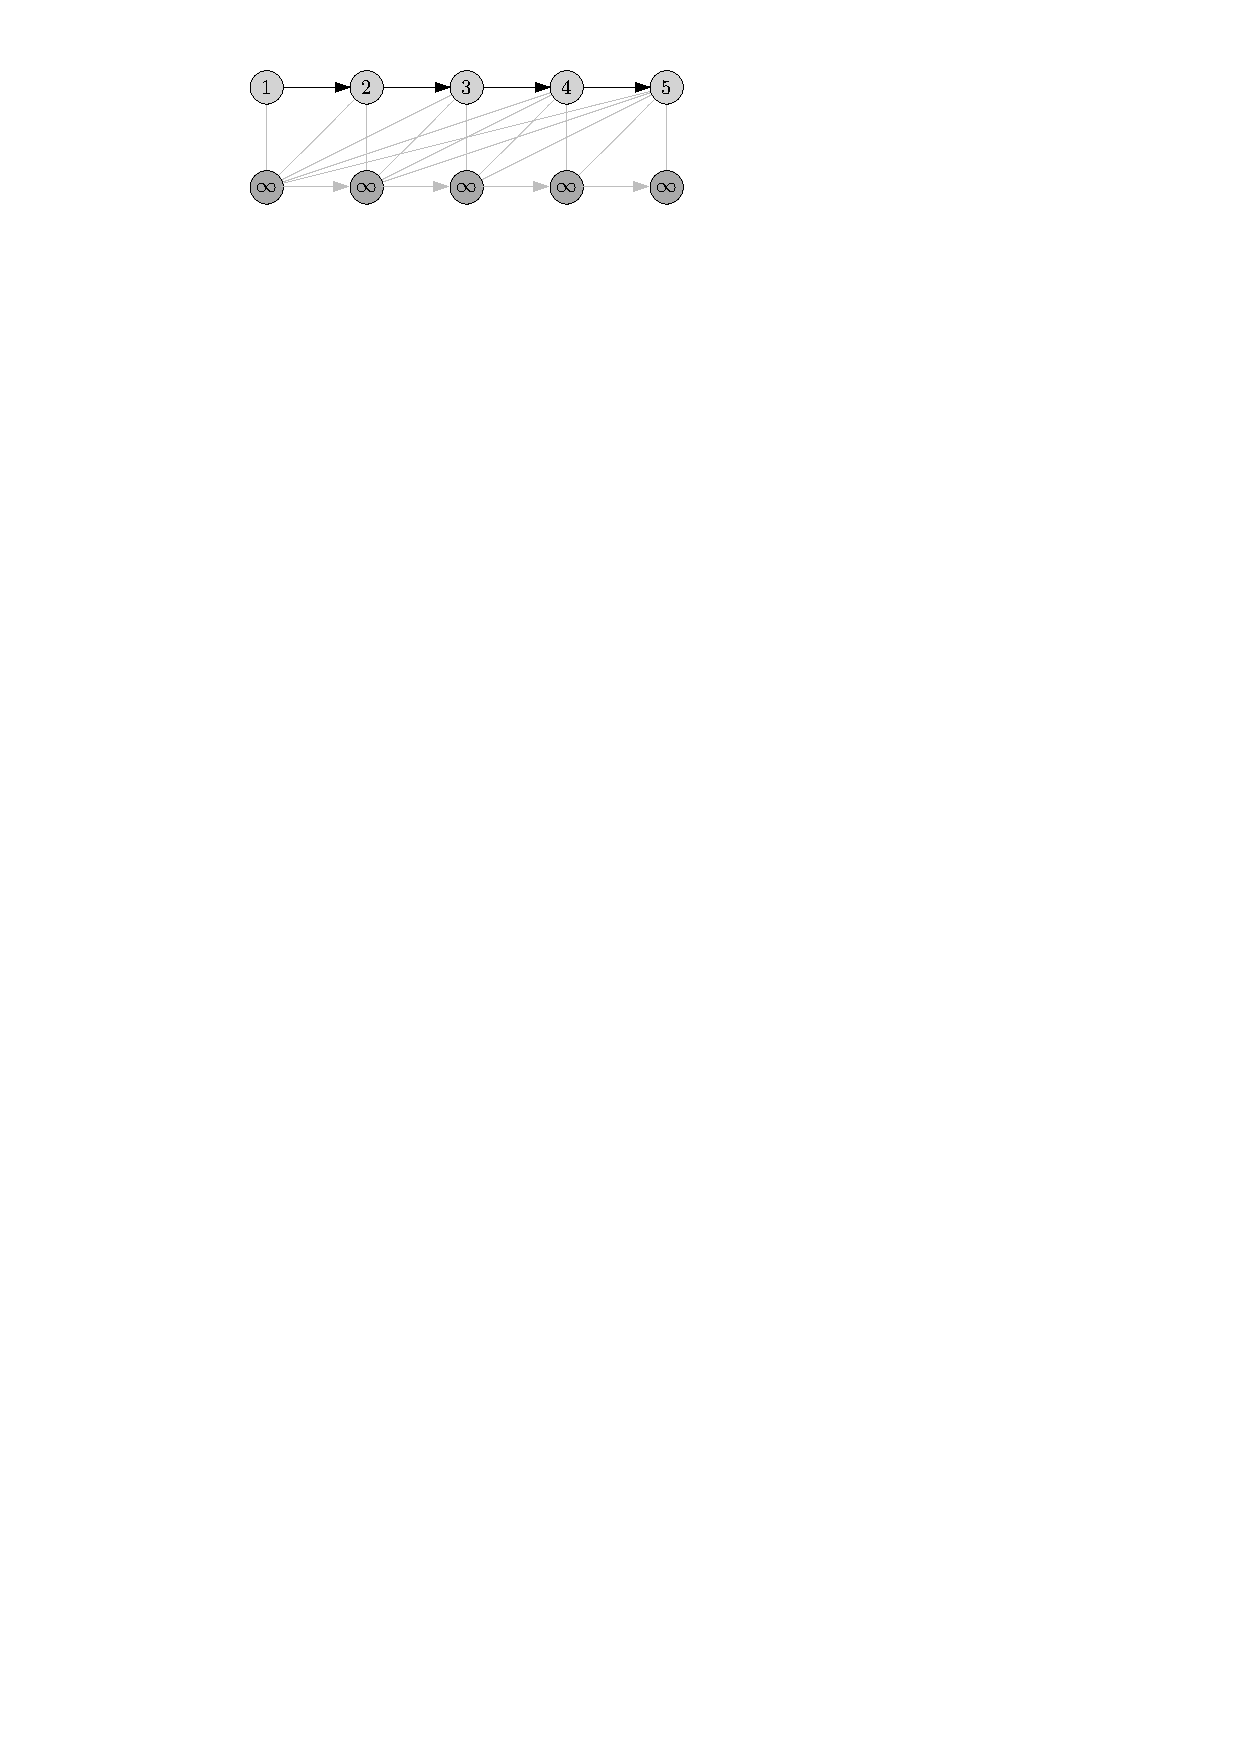
\includegraphics{figures/somegraph}
%   \caption{A funny graph.}
%   \label{fig:somegraph}
% \end{figure}